\documentclass[]{beamer}
\usetheme{Dresden}
% \useoutertheme{split}

\usepackage[ngerman]{babel}
\usepackage[utf8]{inputenc}
\usepackage{color}
\usepackage{graphicx}
\usepackage{listings}
\usepackage{lmodern} %% allow bold keywords
\usepackage{menukeys}
\usepackage{qtree}

\definecolor{darkgreen}{rgb}{0,0.5,0}
\definecolor{lightblue}{rgb}{0.2,0.2,1}

\lstset{language=Java,
	basicstyle=\ttfamily\footnotesize,
	keywordstyle=\color{purple},
	commentstyle=\color{darkgreen},
	numberstyle=\tiny\color{gray},
	stringstyle=\color{blue},
	tabsize=4,
	showstringspaces=false,
	breaklines=true,
	keepspaces=true,
	numbers=left,
	escapechar=@
}

\title{Java}
\subtitle{Einführung}
\author{FSR Informatik}
\date{\today}

\begin{document}

\section{Organisation}
\begin{frame}
	\titlepage
\end{frame}
\begin{frame}{Overview}
	\tableofcontents
\end{frame}

\subsection{Ablauf}
\begin{frame}{Über diesen Kurs}
	Vorraussetzung
	\begin{itemize}
		\item allgemeine PC Kenntnisse
		\item Programmierkenntnisse in einer anderen Sprache
	\end{itemize}
	Ablauf
	\begin{itemize}
		\item es gibt 10+ Veranstaltungen
	\end{itemize}
\end{frame}

\subsection{Material}
\begin{frame}{Material}
	\begin{itemize}
		\item frage deinen Tutor
		\item tritt der Auditorium Gruppe bei \hfill \\
			\url{http://auditorium.inf.tu-dresden.de}
		\item Übungen und Folien \hfill \\
			\dots fragt euren Tutor
		\item Java Dokumentation \hfill \\
			\url{http://docs.oracle.com/javase/tutorial/java/nutsandbolts/index.html}
	\end{itemize}
\end{frame}

\section{Das erste Programm}
\subsection{Eclipse einrichten}
\begin{frame}{Download}
	Eclipse ist eine mächtige Entwicklungsumgebung\footnote{IDE: Integrated Development Environment} u.A. für Java.
	\begin{itemize}
		\item Versionen für Windows gibt es hier:\\
			\url{http://www.eclipse.org}
		\item nutze deinen Paketmanager unter Linux
	\end{itemize}
	Eclipse ist frei und quelloffen.
\end{frame}

\begin{frame}{Erstelle ein neues Projekt}
	\begin{enumerate}
		\item \menu[,]{File, New, Java Project}
		\item Benenne dein Projekt \dots
		\item \dots und drücke \keys{Finish}
	\end{enumerate}
\end{frame}

\begin{frame}{Beispielprojekt \emph{Hello}}
	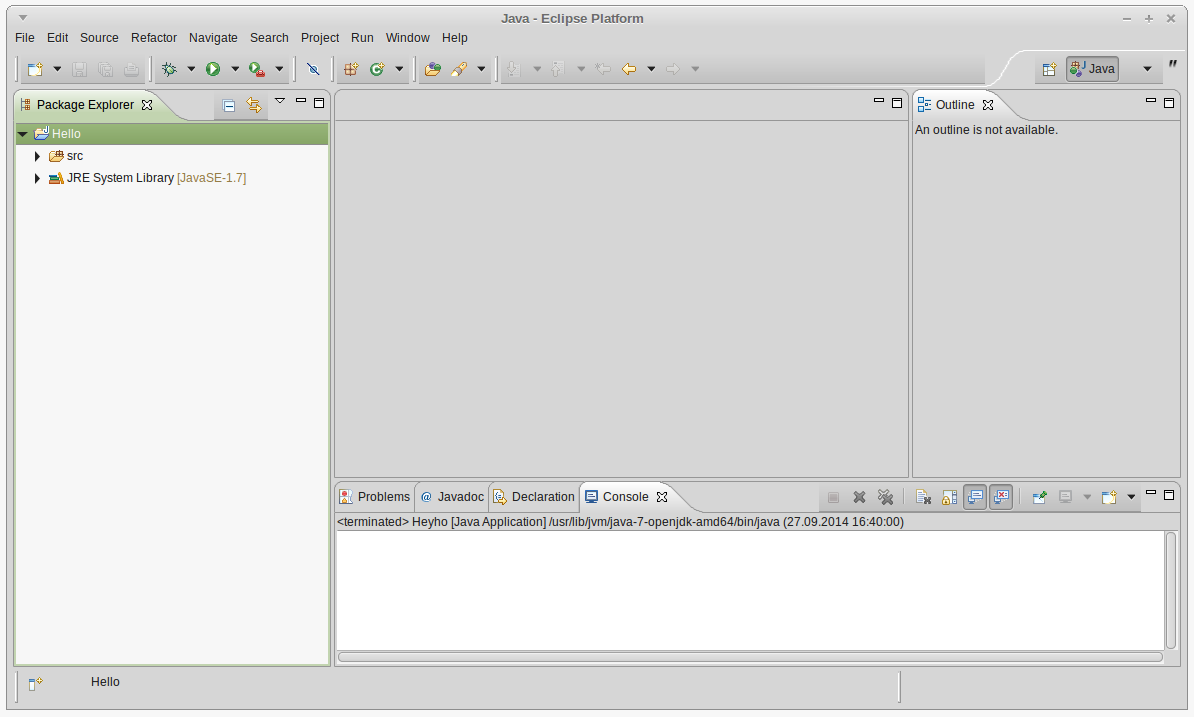
\includegraphics[width=25em]{res/intro_eclipse.png}
\end{frame}

\begin{frame}{Erstelle eine Klasse}
	\begin{enumerate}
		\item Klicke rechts auf dein Projekt im \emph{Package Explorer}. \hfill \\
			\menu[,]{New, Class}
		\item Benenne deine Klasse \dots \\
			\emph{Klassennamen fangen immer mit großen Buchstaben an.}
		\item \dots und drücke \keys{Finish}.
	\end{enumerate}
\end{frame}

\subsection{Hello World!}

\begin{frame}[fragile]{Hello World!}
	Eclipse generiert folgende leere Klasse:
	\begin{lstlisting}
	public class Hello {
	
	}
	\end{lstlisting}
\end{frame}

\begin{frame}[fragile]{Hello World!}
	Dieses Programm gibt \emph{Hello World!} auf der Konsole aus:
	\begin{lstlisting}
	public class Hello {
	    public static void main(String[] args) {
	        System.out.println("Hello World!");
	    }
	}
	\end{lstlisting}
\end{frame}

\begin{frame}[fragile]{Hello World!}
	\begin{lstlisting}
	public class Hello {
	    public static void main(String[] args) {
	        System.out.println("Hello World!");
	    }
	}
	\end{lstlisting}
	Starte das Programm mit dem grünen Knopf:\\
	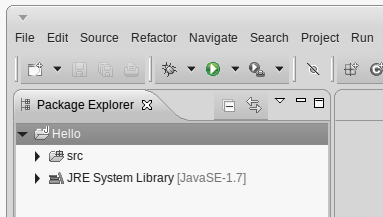
\includegraphics[width=10em]{res/intro_run.png} \\
	oder drücke \keys{\ctrl + F11}.
\end{frame}

\begin{frame}[fragile]{Kommentare}
	\begin{lstlisting}
	public class Hello {
	    // prints a "Hello World!" on your console
	    public static void main(String[] args) {
	        System.out.println("Hello World!");
	    }
	}
	\end{lstlisting}
	Kommentiere immer deinen Quelltex. \\
	Quelltext wird häufiger gelesen als geschrieben.
	\begin{itemize}
		\item // einzelne Kommentarzeile
		\item /* Kommentar verteilt über \\
			mehrere Zeilen */
	\end{itemize}
\end{frame}

\section{Grundlagen}
\subsection{Definitionen}

\begin{frame}{primitive Datentypen}
	Java unterstützt mehrere \textbf{primitive Datentypen}:
	\begin{itemize}
		\item[boolean] ein Wahrheitswert (entweder \textbf{true} oder \textbf{false})
		\item[int] eine 32 bit Ganzzahl
		\item[long] eine 64 bit Ganzzahl
		\item[float] eine 32 bit Fließkommazahl
		\item[double] eine 64 bit Fließkommazahl
		\item[char] ein ascii Zeichen
		\item[void] der leere Typ (wird später behandelt)
	\end{itemize}
\end{frame}

\begin{frame}[fragile]{Blöcke}
	\begin{lstlisting}
	public class Hello @\textcolor{red}{\texttt{\{}}@
	    // prints a "Hello World!" on your console
	    public static void main(String[] args) {
	        System.out.println("Hello World!");
	    }
	@\textcolor{red}{\texttt{\}}}@
	\end{lstlisting}
	Alles zwischen \{ und \} ist ein \emph{Block}. \\
	Blöcke können geschachtelt werden.
\end{frame}

\begin{frame}[fragile]{Semikolons}
	\begin{lstlisting}
	public class Hello {
	    // prints a "Hello World!" on your console
	    public static void main(String[] args) {
	        System.out.println("Hello World!")@\textcolor{red}{\texttt{;}}@
	    }
	}
	\end{lstlisting}
	Semikolons schließen Befehle ab. \\
	Blöcke müssen nicht mit Semikolons abgeschlossen werden.
\end{frame}

\begin{frame}[fragile]{Variablennamen}
	\begin{itemize}
		\item Variablennamen beginnen mit beliebigen Buchstaben oder Unterstrich.
		\item Zusammengesetzte Namen sollten BinnenMajuskel\footnote{engl: CamelCase} verwenden.
		\item Variablen sollten ihrer Bedeutung entsprechend benannt werden.
	\end{itemize}
	\begin{lstlisting}
	public static void main(String[] args) {
	    	int a = 0; // not very meaningful
	    	float myFloat = 5.3f; // also not meaningful
	    	int count = 7; // quite a good name
	    	
	    	int rotationCount = 7; // there you go
	}
	\end{lstlisting}
\end{frame}

\subsection{Rechenoperationen}

\begin{frame}[fragile, allowframebreaks]{Rechnen mit \emph{int}}
	\begin{lstlisting}
	public class Calc {
	    public static void main(String[] args) {
	        int a; // declare variable a
	        a = 7; // assign 7 to variable a
	        System.out.println(a); // prints: 7
	        a = 8;
	        System.out.println(a); // prints: 8
	        a = a + 2;
	        System.out.println(a); // prints: 10
	    }
	}
	\end{lstlisting}
	Nach der Deklaration wird der Variable ein Wert zugewiesen.
\framebreak
	\begin{lstlisting}
	public class Calc {
	    public static void main(String[] args) {
	        int a = -9; // declaration and assignment of a
	        int b; // declaration of b
	        b = a; // assignment of b
	        System.out.println(a); // prints: -9
	        System.out.println(b); // prints: -9
	        a++; // increments a
	        System.out.println(a); // prints: -8
	    }
	}
	\end{lstlisting}
	\textbf{Deklaration} und \textbf{Zuweisung} können gleichzeitig stattfinden.
\framebreak
	\begin{lstlisting}
	public class Calc {
	    public static void main(String[] args) {
	        int b; // declaration of b
	        System.out.println(b);
	    }
	}
	\end{lstlisting}
	Variablen ohne Zuweisung verursachen Exceptions.\\
	Exceptions sind Fehler, die später im Laufe des Kurses erklärt werden.
	\vspace{1em}
	\emph{Weise deinen Variablen immer einen Wert zu!}
\framebreak
	%linebreak is intended

	Einige mathematische Operationen:
	\begin{tabular}{ll}
		Addition & \texttt{a + b;} \\
		Subtraktion & \texttt{a - b;} \\
		Multiplikation &\texttt{a * b;} \\
		Division & \texttt{a / b;} \\
		Modulo & \texttt{a \% b;} \\
		Inkrement & \texttt{a++;} \\
		Dekrement & \texttt{a--;} \\
	\end{tabular}
\end{frame}

\begin{frame}[fragile, allowframebreaks]{Rechnen mit \emph{float}}
	\begin{lstlisting}
	public class Calc {
	    public static void main(String[] args) {
	        float a = 9;
	        float b = 7.5f;
	        System.out.println(a); // prints: 9.0
	        System.out.println(b); // prints: 7.5
	        System.out.println(a + b); // prints: 16.5
	    }
	}
	\end{lstlisting}
\framebreak
	\begin{lstlisting}
	public class Calc {
	    public static void main(String[] args) {
	        float a =       8.9f;
	        float b = 3054062.5f;
	        System.out.println(a); // prints: 8.9
	        System.out.println(b); // prints: 3054062.5
	        System.out.println(a + b); // prints: 3054071.5
	    }
	}
	\end{lstlisting}
	Float hat begrenzte Genauigkeit. \\
	\emph{Dies kann zu unerwarteten Ergebnissen führen!}
\end{frame}

\begin{frame}[fragile]{Rechnen mit \emph{int} und \emph{float}}
	\begin{lstlisting}
	public class Calc {
	    public static void main(String[] args) {
	        float a = 9.3f;
	        int b = 3;
	        System.out.println(a + b); // prints: 12.3
	        float c = a + b;
	        System.out.println(c); // prints: 12.3
	    }
	}
	\end{lstlisting}
	Java konvertiert \textbf{int} zu \textbf{float}, wenn notwenig. \\
	Umgekehrt gilt das nicht.
\end{frame}

\subsection{Text mit Zeichenketten}

\begin{frame}[fragile]{Strings}
	String\footnote{deu: Zeichenkette} ist kein primitiver Datentyp, sondern ein Objekt Typ. \\
	Objekt Typen werden in der nächsten Veranstaltung erklärt.
	\begin{lstlisting}
	public class Calc {
	    public static void main(String[] args) {
	        String hello = "Hello World!";
	        System.out.println(hello); // print: Hello World!
	    }
	}
	\end{lstlisting}
\end{frame}

\begin{frame}[fragile]{Verketten}
	\begin{lstlisting}
	public class Calc {
	    public static void main(String[] args) {
	        String hello = "Hello";
	        String world = " World!";
	        String sentence = hello + world;
	        System.out.println(sentence);
	        System.out.println(hello + " World!");
	    }
	}
	\end{lstlisting}
	Strings können mit + verkettet werden. 
	Im Beispiel wird zweimal die gleiche Zeile ausgegeben.
\end{frame}

\begin{frame}[fragile]{Strings und Zahlen}
	\begin{lstlisting}
	public class Calc {
	    public static void main(String[] args) {
	    	int factorA = 3;
	    	int factorB = 7;
	    	int product = factorA * factorB;
	    	String answer = 
	            factorA + " * " + factorB + " = " + product;
	        System.out.println(answer); // prints: 3 * 7 = 21
	    }
	}
	\end{lstlisting}
	Wenn Strings mit primitiven Typen verkettet werden, wird der primitive Datentyp,
	entsprechend seiner Zuweisung, in ein String übersetzt und verkettet.
\end{frame}

\end{document}